\documentclass[eng,printmode,oneside]{mgr}
\usepackage[MeX]{polski}
\usepackage[utf8]{inputenc}
\usepackage[T1]{fontenc} 
\usepackage{graphicx}
\usepackage{subfigure}
\usepackage{psfrag}
\usepackage{amsmath}
\usepackage{amsfonts}
%\usepackage{supertabular}
\usepackage{array}
\usepackage{tabularx}
\usepackage{hhline}
\usepackage{rev}
%\usepackage{framed}
\usepackage{color}
\usepackage{url}
%\usepackage[notref]{showkeys}
%\usepackage{showlabels}
\usepackage{float}
%\usepackage{tikz}
\usepackage{enumitem} 
\usepackage{graphicx}       
\usepackage{rotating}       % pakiet umożliwiający obracanie rysunków
\usepackage{subfigure}      % pakiet umożliwiający tworzenie podrysunków
\usepackage{epic}           
\usepackage{listings}       % pakiet dedykowany zrodlom programow
\usepackage{verbatim}       % pakiet dedykowany rozmaitym wydrukom tekstowym
\usepackage{amssymb}        % pakiet z rozmaitymi symbolami matematycznymi
\usepackage{amsmath}        % pakiet z rozmaitymi środowiskami matematycznymi
\usepackage[polish]{babel}  % pakiet lokalizujący dokument w języku polskim
\usepackage[OT4]{fontenc}
\usepackage[utf8]{inputenc}
\usepackage{bm}
\usepackage{gensymb}
\usepackage{booktabs}
\usepackage{epstopdf}
\usepackage{amssymb}
\usepackage[utf8]{inputenc}
\usepackage{amsmath}
\usepackage{amsfonts}
\usepackage{amssymb}
\usepackage{graphics}
\usepackage[]{algorithmic} %pseudocode
\usepackage[]{algorithm2e} %pseudocode
\usepackage{float}
\usepackage{csquotes}
\usepackage{epsfig}
%\usepackage{hyperref}
\usepackage{wrapfig} 
\reviewer{dypl}{0.2}{0.2}{0.67}
\reviewer{prof}{0.2}{0.6}{0.2}
\def\bp{\begin{review}[prof]}
\def\ep{\end{review}}
\def\bdypl{\begin{review}[dypl]}
\def\edypl{\end{review}}
\newcommand{\R}{I\!\!R} 
\newtheorem{theorem}{Twierdzenie}[section] 
\newcommand\numberthis{\addtocounter{equation}{1}\tag{\theequation}}
\newenvironment{myitemize}%
 { \begin{list}{\labelitemi}%
   {
      \setlength{\itemsep}{0mm}%
      \setlength{\topsep}{6pt}%
      \setlength{\leftmargin}{5mm}%
     \setlength{\parsep}{1mm}%
    }
  }
{\end{list}
}
\newcounter{mycount}
\newenvironment{MYenumerate}%
 {\begin{list}{\arabic{mycount}.}%
   {\usecounter{mycount}%
%      \setlength{\topsep}{12pt}%
      \setlength{\topsep}{6pt}%
      \setlength{\itemsep}{0mm}%
      \setlength{\leftmargin}{7mm}%
     \setlength{\parsep}{1mm}%
    }%
 }%
{\end{list}}
\newenvironment{todo}
{
\label{todo}
\color{red} [
}
{]
}
%%%%%%%%%chapter no new page%
\usepackage{etoolbox}

\makeatletter
\patchcmd{\chapter}{\if@openright\cleardoublepage\else\clearpage\fi}{}{}{}
\makeatother
%%%%%%%%%%%%%
\title{?}
\engtitle{?}

\author{inż. Bernard Malec}
\supervisor{Prof.\ dr hab.\ inż.\ Alicja Mazur}


\field{Automatyka i Robotyka (AIR)}
\specialisation{Robotyka (ARR)}

%\includeonly{mch0,mch1,mch2,mch3,mch4,bibl}
%\includeonly{mch3}

\begin{document}
\bibliographystyle{plabbrv} %BibTeX polski styl bibliografii 

% te ozdobniki dodaje się dopiero na końcu 
%\maketitle

\chapter{Model satelity typu free-floating}
\section{Model we współrzędnych uogólnionych}
Robot free-floating z manipulatorem to nienapędzana platforma (baza) z zamontowanym na niej napędzanym manipulatorem. Robot taki znajduje się w przestrzeni kosmicznej w stanie mikrograwitacji (nieważkości).
\par W rozważanym robocie platformą będzie jednolita prostokątna płyta, a za manipulator posłuży manipulator RR. Rozważanego robota free-floating z manipulatorem przedstawiono na rys 1. \par Robot taki jest użyteczny ze względów praktycznych. Do badań eksperymentalnych bowiem, można wykorzystać płaską granitową płytę, po której baza może ślizgać się bez tarcia. %, a siły grawitacji nie mają wpływu na dynamikę.
Dzięki temu testy można przeprowadzać na Ziemi, a nie w warunkach mikrograwitacji.

\par Do wyprowadzenia modelu we współrzędnych uogólnionych weźmy następujące współrzędne
\begin{equation}
q=\left(
\begin{array}{c}
q_b\\
q_r\\
\end{array}
\right),
\end{equation}
gdzie $q_b=(x,y,\theta)^T$ -- wektor współrzędnych uogólnionych bazy, $q_r=(q_1,q_2)^T$ -- wektor współrzędnych przegubowych manipulatora. 
\par Równania dynamiki we współrzędnych uogólnionych takiego robota można, ponownie korzystając z formalizmu Langrange'a, zapisać jako\\
\begin{equation}
\label{wrsdad}
H(q)\ddot{q}+C(q,\dot{q})\dot{q}=
\left(
\begin{array}{c}
0\\
u\\
\end{array}
\right).
\end{equation}\\
Brak wektora sił potencjalncyh $D(q)$ wynika z braku grawitacji. \par Sterowanie $u$ pojawia się tylko w dolnej części równania dynamiki (\ref{wrsdad}), ponieważ dotyczy jedynie manipulatora, jako że baza jest nienapędzana (free-floating).

%\end{equation}\\
\section{Model we współrzędnych barycentrycznych}
Jeśli środek masy robota free-floating z manipulatorem ma pozostać nieruchomy (lub poruszać się ze stałą prędkością), konieczne jest zamodelowanie dynamiki we współrzędnych barycentrycznych.\\
\par Położenie środka masy robota free-floating z manipulatorem można wyliczyć z definicji jako
\begin{equation}
\left(\sum\limits^w_{i=1}m_i\right)\phi_b=\sum\limits^w_{i=1}m_ir_i,
\end{equation}
gdzie $r_i$ to środek masy $i$-tego członu robota w podstawowym układzie współrzędnych, a  $m_i$ to masa $i$-tego członu. Z kolei $w$ to liczba członów robota. W naszym przypadku $w$ wynosi trzy, robot posiada bowiem jedną bazę i dwa ramiona.\\
$\phi_b$ to współrzędne barycentryczne układu, czyli
\begin{equation}
\label{baro}
\phi_b=
\left(
\begin{array}{c}
\bar{x}\\
\bar{y}\\
\theta\\
\end{array}
\right)=
\frac{\sum\limits^w_{i=1}m_ir_i}{\sum\limits^w_{i=1}m_i}.
\end{equation}
Kompletne współrzędne barycentryczne satelity wraz z manipulatorem $\phi$ mają postać
\begin{equation}
\phi=
\left(
\begin{array}{c}
\phi_b\\
q_r\\
\end{array}
\right).
\end{equation}
Model we współrzędnych barycentrycznych można więc wyrazić jako
\begin{equation}
\bar{H}\ddot{\phi}+\bar{C}\dot{\phi}
=
\left(
\begin{array}{c}
0\\
u\\
\end{array}
\right),
\end{equation}
%\bar{H}\ddot{\phi}+\bar{c}
%=
%\begin{bmatrix}
%    \bar{H}_b  &\bar{H}_{bm}\\
%    \bar{H}_{bm}^T  &\bar{H}_m \\
%\end{bmatrix}
%\left(
%\begin{array}{c}
%\ddot{\phi_b}\\
%\ddot{q_m}\\
%\end{array}
%\right)
%+
%\left(
%\begin{array}{c}
%\bar{c}_b\\
%\bar{c}_m\\
%\end{array}
%\right)
%=
%\left(
%\begin{array}{c}
%0\\
%u\\
%\end{array}
%\right),
%\end{equation}

Macierze $\bar{H}$ i $\bar{C}$ uzyskuje się przez przeliczenie energii kinetycznej do układu współrzędnych barycentrycznych i wykorzystanie formalizmu Lagrange'a dla nowej energii kinetycznej.\\

\chapter{Odsprzęganie wejściowo-wyjściowe dla robota free-floating z manipulatorem}

Ponieważ baza robota free-floating z manipulatorem nie jest napędzana, do odsprzęgania wejściowo-wyjściowego nie można zastosować podstawowego algorytmu Yamamoto i Yuna. Do realizacji zadania śledzenia trajektorii w przestrzeni zadaniowej wykorzystamy więc algorytm z rozszerzonymi funkcjami wyjściowymi.
\par Algorytm ten można stosować zarówno dla modelu robota free-floating z manipulatorem we współrzędnych uogólnionych, jak i we współrzędnych barycentrycznych. Wybór modelu należy podporządkować rodzajowi zadania, jakie ma zostać wykonane. Jeśli środek masy ma pozostać nieruchomy wykorzystać należy model we współrzędnych barycentrycznych, natomiast gdy środek masy ma się przemieszczać, to można użyć modelu we współrzędnych uogólnionych.
\par Przy wyprowadzaniu algorytmu wykorzystamy model dynamiki we współrzędnych uogólnionych. Algorytm dla modelu we współrzędnych barycentrycznych wyprowadza się analogicznie, podstawiając jedynie za współrzędne uogólnione $q$ i macierze  $H$ i $C$ oraz ich odpowiedniki w modelu we współrzędnych barycentrycznych, tj.  współrzędne barycentryczne $\phi$ i macierze $\bar{H}$ i $\bar{C}$.

\par Korzystamy z algorytmu z rozszerzonymi funkcjami wyjściowymi, więc postać funkcji wyjściowej będzie zależeć od całej konfiguracji $q$:
\begin{equation}
y=k(q).
\end{equation}
\section{Algorytm odsprzęgania wejściowo-wyjściowego}
Przy wyprowadzaniu algorytmów odsprzęgania wejściowo-wyjściowego dla manipulatora mobilnego linearyzowaliśmy jego dynamikę w celu ułatwienia obliczeń. W przypadku robota free-floating z manipulatorem linearyzacja taka jest kłopotliwa, ponieważ tylko manipulator jest napędzany. Aby nie utrudniać sobie zadania i pokazać, że linearyzacja dynamiki nie jest konieczna, nie zastosujemy jej przy wyprowadzaniu algorytmu odsprzęgania wejściowo-wyjściowego dla robota free-floating z manipulatorem.
\par Struktura algorytmu nie zmienia się i nadal składa się z dwóch pętli sprzężenia zwrotnego: pierwsza przekształca układ do postaci liniowej typu "podwójny integrator", druga steruje uzyskanym układem liniowym.
\par Prawo sterowania pierwszej pętli wyprowadza się analogicznie, jak w przypadku manipulatorów mobilnych.
Niech $y_i=k_i(q)$ oznacza $i$-tą współrzędną chwytaka satelity, wyrażoną względem układu podstawowego. Oczywiste jest, że $i=1,...,p$, gdzie $p\leq6$.
\par Zróżniczkujmy wszystkie elementy wektora $y(q)$ dwukrotnie po czasie
\begin{equation}
\dot{y}_i=\dfrac{d}{dt}\left(k_i(q)\right)=\dfrac{\partial k_i(q)}{\partial q}\dot{q}=J_i\dot{q},
\end{equation}
\begin{equation}
\ddot{y}_i=\dot{q}^T\dfrac{\partial^2k_i(q)}{\partial q^2}\dot{q}+J_i\ddot{q}=P_i+J_i\ddot{q},
\end{equation}
gdzie
\begin{equation}
J_i=\dfrac{\partial k_i(q)}{\partial q},
\end{equation}
\begin{equation}
P_i=\dot{q}^T\dfrac{\partial^2k_i(q)}{\partial q^2}\dot{q}.
\end{equation}
Zapiszmy $\dot{y}$ i $\ddot{y}$ w postaci wektorowej
\begin{equation}
\dot{y}=J\dot{q},
\end{equation}
\begin{equation}
\label{ypplol}
\ddot{y}=P+J\ddot{q},
\end{equation}
gdzie
\begin{equation}
P=
\left(
\begin{array}{c}
P_1\\
P_2\\
\vdots\\
P_p\\
\end{array}
\right),
\end{equation}
\begin{equation}
J=
\left(
\begin{array}{c}
J_1\\
J_2\\
\vdots\\
J_p\\
\end{array}
\right),
\end{equation}
$p$ jest liczbą zmiennych wyjściowych $y$.
\par Korzystając z dynamiki we współrzędnych uogólnionych (\ref{wrsdad}), zapiszmy $\ddot{q}$  jako
\begin{equation}
\label{qpplol}
\ddot{q}=H^{-1}
\left[
\left(
\begin{array}{c}
0\\
u\\
\end{array}
\right)
-C\dot{q}
\right].
\end{equation}
Podstawmy teraz  (\ref{qpplol}) do (\ref{ypplol})
\begin{equation}
\ddot{y}=P+J
H^{-1}
\left[
\left(
\begin{array}{c}
0\\
u\\
\end{array}
\right)
-C\dot{q}
\right],
\end{equation}
a otrzymamy równanie o postaci
\begin{equation}
\ddot{y}=
P-JH^{-1}C\dot{q}
+
JH^{-1}\left(
\begin{array}{c}
0\\
u\\
\end{array}
\right).
\end{equation}
Zapiszmy więc $\ddot{y}$ następująco
\begin{equation}
\ddot{y}=
F+G\left(\begin{array}{c}
0\\
u\\
\end{array}
\right),
\end{equation}
gdzie
\begin{equation}
F=P-JH^{-1}C\dot{q},
\end{equation}
\begin{equation}
G=JH^{-1}.
\end{equation}
macierz $G$ zapiszmy jako $G=[G_1|G_2]$. Macierz $G_2$ jest rozmiaru $p\times p$.\\
Wektor $\ddot{y}$ można zapisać wtedy jako
\begin{equation}
\label{helloasdasda}
\ddot{y}=F+G_2u.
\end{equation}
Prawo sterowania pętli linearyzującej jest następujące
\begin{equation}
\label{ulol}
u=G_2^{-1}(-F+\zeta),
\end{equation}
przy czym symbolem $\zeta$ oznaczono nowe wejście do układu.
Podstawiając (\ref{ulol}) do (\ref{helloasdasda}) otrzymujemy równanie układu z zamkniętą pętlą sprzężenia zwrotnego
\begin{equation}
\label{helloasdasdaasdasdasd}
\ddot{y}=\zeta.
\end{equation}
Jak widać, jest to układ liniowy typu "podwójny integrator".
Za wysterowanie go odpowiada druga pętla. Zrealizować ją, można np. jako regulator PD z korekcją (\ref{PD}).

\subsection{Badania symulacyjne}
Podrozdział ten jest poświęcony symulacji algorytmu odsprzęgania wejściowo-wyjściowego dla robota free-floating z manipulatorem.\\
\par Algorytm zbadano na przedstawionym w pracy modelu dynamiki we współrzędnych barycentrycznych. \\
\par Parametry geometryczne i masowe ustalono jako: $l_1$=1m, $l_2$=1m, $m_0=$20kg, $m_1$=$m_2$=10kg.\\
Początkowa konfiguracja manipulatora była równa 
\begin{center}
$q_r(0)=
\left(
\begin{array}{c}
   0 \\
    0.1 \\
\end{array}
\right).$
\end{center}
Początkową konfigurację bazy $q_b(0)$ we współrzędnych uogólnionych ustalono jako
\begin{center}
$q_b(0)=
\left(
\begin{array}{c}
   x(0) \\
    y(0) \\
    \theta(0)\\
\end{array}
\right)=
\left(
\begin{array}{c}
    0 \\
     0 \\
     0 \\
\end{array}
\right),$
\end{center}
co odpowiada następującej konfiguracji początkowej bazy we współrzędnych barycentrycznych
\begin{center}
$\phi_b(0)=
\left(
\begin{array}{c}
   \bar{x}(0) \\
   \bar{y}(0) \\
    \theta(0)\\
\end{array}
\right)=
\left(
\begin{array}{c}
    0.4994 \\
     0.0125 \\
     0\\
\end{array}
\right).$
\end{center}
Wynika to z przekształcenia (\ref{baro}). W naszym wypadku $\bar{x}$ i $\bar{y}$ są równe
\begin{center}$
\begin{array}{c}
\bar{x}= \dfrac{{m_2} \left({l_1}
   c_{01}+\dfrac{1}{2} {l_2} c_{012}\right)}{{m_1}+{m_2}+{m_0}}+\dfrac{{l_1} {m_1} c_{01}}{2   ({m_1}+{m_2}+{m_0})}+x,\\
   \bar{y}= \dfrac{{m_2} \left({l_1} s_{01}+\dfrac{1}{2} {l_2} s_{012}\right)}{{m_1}+{m_2}+{m_0}}+\dfrac{{l_1} {m_1} s_{01}}{2
   ({m_1}+{m_2}+{m_0})}+y.
   \end{array}
$\end{center}
Prędkości początkowe były równe
\begin{center}
$\dot{q}_r(0)=
\left(
\begin{array}{c}
    0 \\
     -0.1\\
\end{array}
\right),$
\end{center}
\begin{center}
$\dot{q}_b(0)=
\left(
\begin{array}{c}
    0 \\
     0 \\
     0.2\\
\end{array}
\right),$
\end{center}
\begin{center}
$\dot{\phi}_b(0)=
\left(
\begin{array}{c}
    -0.0012 \\
     0.0874 \\
     0.2\\
\end{array}
\right),$
\end{center}
\par Konieczne jest, aby liczba sterowań była równa liczbie wyjść. Wówczas sterować można dwoma przegubami manipulatora, a więc możliwe jest odsprzęgnięcie dwóch współrzędnych efektora. Wybrano współrzędne $x$ i $y$ efektora w podstawowym układzie odniesienia ($X_0$,$Y_0$).\\
Funkcja wyjścia $y$ ma postać
\begin{center}
$y(t)=y(q_b,q_r)=y(\phi_b,q_r)=
\left(
\begin{array}{c}
    x + l_1c_{01} + l_2c_{012}\\
    y + l_1s_{01} + l_2s_{012}\\
\end{array}
\right)=$
$=\left(
\begin{array}{c}
   \dfrac{{l_1} ({m_1}+2  {m_0}) c_{01}+ {l_2} (2
    {m_1}+ {m_2}+2  {m_0}) c_{012}+2  \bar{x}
   ( {m_1}+ {m_2}+ {m_0})}{2( {m_1}+ {m_2}+ {m_0})}\\\\
   \dfrac{ {l_1}   ( {m_1}+2  {m_0}) s_{01}+ {l_2} (2  {m_1}+ {m_2}+2
    {m_0}) s_{012}+2    \bar{y} ( {m_1}+ {m_2}+ {m_0})}{2
   ( {m_1}+ {m_2}+ {m_0})}
\end{array}
\right).$
\end{center}
Funkcje wyjścia miały następujące wartości początkowe 
\begin{center}
$y(0)=y(q_b(0),q_r(0))=y(\phi_b(0),q_r(0))=
\left(
\begin{array}{c}
     1.9950 \\
     0.0998 \\
\end{array}
\right).$
\end{center}
Prędkości chwytaka w chwili początkowej były równe
\begin{center}
$\dot{y}(0)=
\left(
\begin{array}{c}
    -0.0100 \\
     0.2995 \\
\end{array}
\right).$
\end{center}
Wybrano następujące trajektorie zadane $y_d(t)$ 
\begin{center}
$y_d(t)=
\left(
\begin{array}{c}
    0.2\sin(0.2t)\\
   1+0.01\ln(30(t+1))\\
\end{array}
\right).$
\end{center}
Błąd początkowy $e(t)=y_d(t)-y(t)$ i jego pochodna były równe
\begin{center}
$e(0)=
\left(
\begin{array}{c}
   -1.9950\\
    0.9342\\
   \end{array}
\right), \hspace{1.5cm}
\dot{e}(0)=
\left(
\begin{array}{c}
    0.0500\\
    -0.2895\\
\end{array}
\right).$
\end{center}
Do sterowania układem liniowym użyto regulatora PD z korekcją (\ref{PD}) z nastawami $K_d=4$, $K_p=2$.
W badaniach raz jeszcze wykorzystano środowisko Matlab/Simulink. \\
Rezultaty badań przedstawiono poniżej.

\begin{figure}[H]
\centering
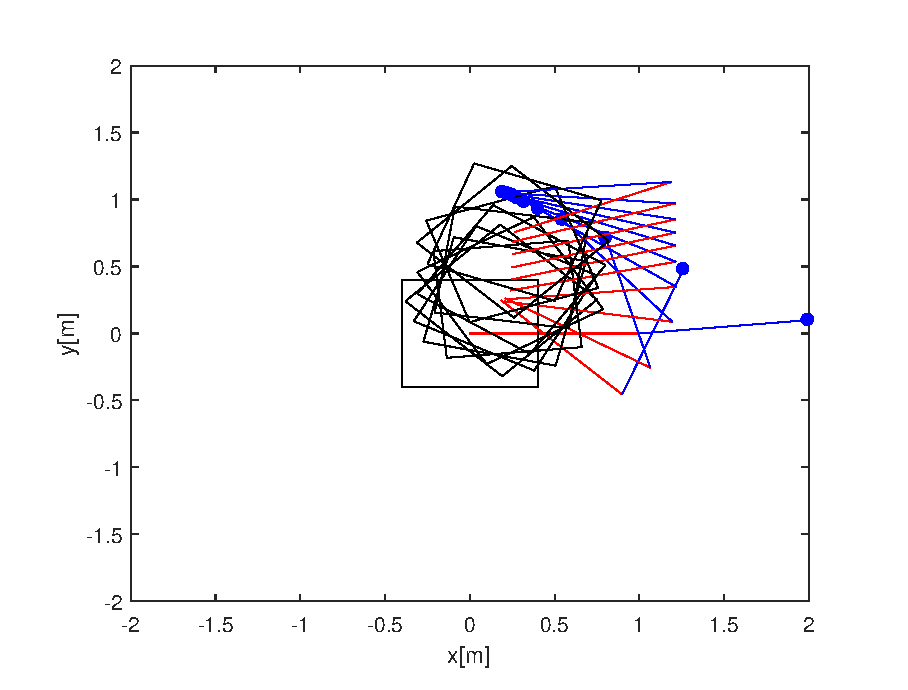
\includegraphics[width=.8\linewidth]{pics/FF1BaryDrawing}
\caption{Robot free-floating z manipulatorem w kolejnych chwilach czasu}
\label{fig:FF1Drawing}
\end{figure}

Przebiegi błędów śledzenia trajektorii chwytaka pokazano na rys. \ref{fig:FF1Barye}
\begin{figure}[H]
\centering
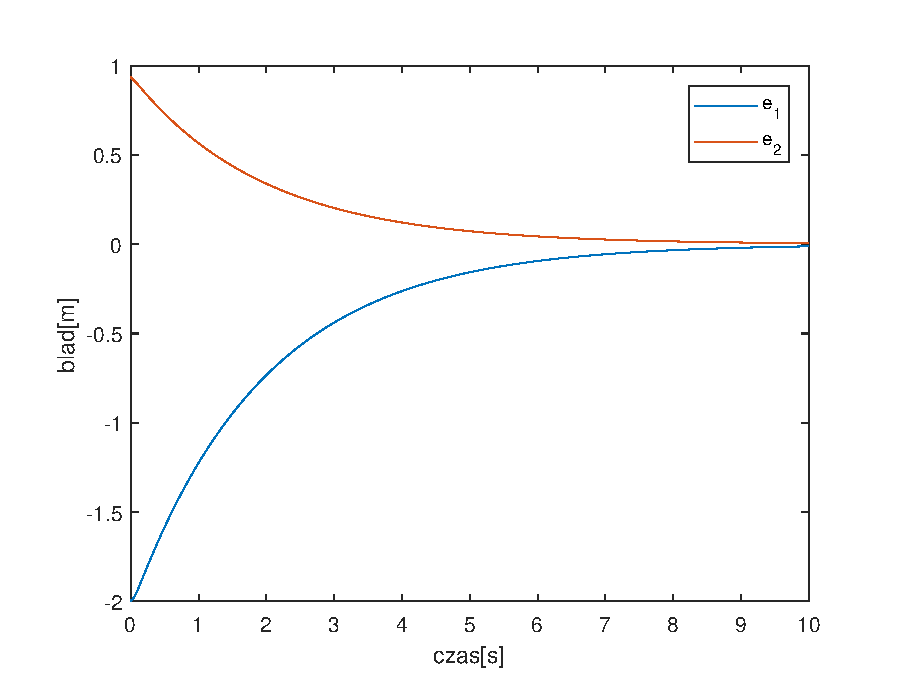
\includegraphics[width=.6\linewidth]{pics/FF1Barye}
\caption{Przebiegi błędów śledzenia trajektorii chwytaka}
\label{fig:FF1Barye}
\end{figure}

Przebiegi współrzędnych uogólnionych $q_b$ i $q_r$ pokazano na rys. \ref{fig:FF1BaryQ}
\begin{figure}[H]
\centering 
\begin{minipage}{.5\textwidth}
  	\centering
  	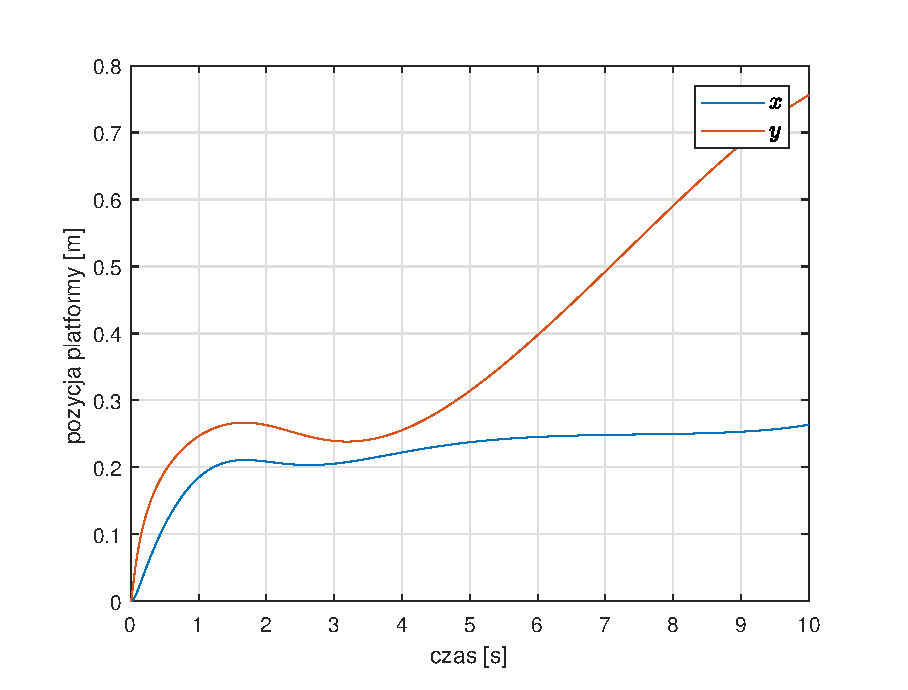
\includegraphics[width=.99\linewidth]{pics/FF1BaryX}
\end{minipage}%
\begin{minipage}{.5\textwidth}
 	\centering
    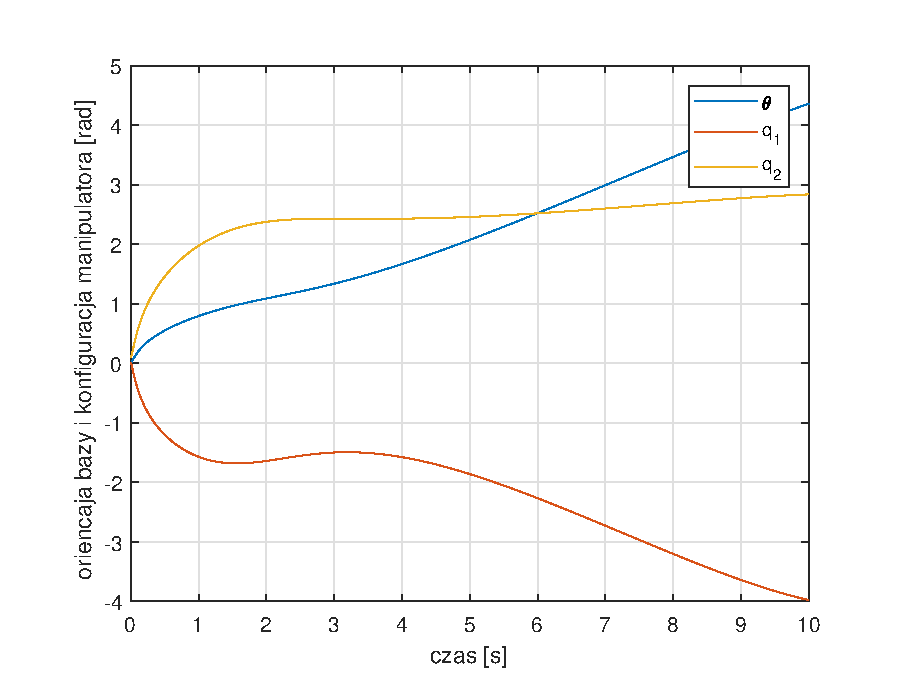
\includegraphics[width=.99\linewidth]{pics/FF1BaryQ}
\end{minipage}%
\caption{Przebiegi współrzędnych uogólnionych $q_b$ i $q_r$}
\label{fig:FF1BaryQ}
\end{figure}

Przebiegi współrzędnych barycentrycznych $\bar{x}$ i $\bar{y}$ i ich prędkości pokazano na rys. \ref{fig:FF1BaryXBAR}
\begin{figure}[H]
\centering 
\begin{minipage}{.5\textwidth}
  	\centering
  	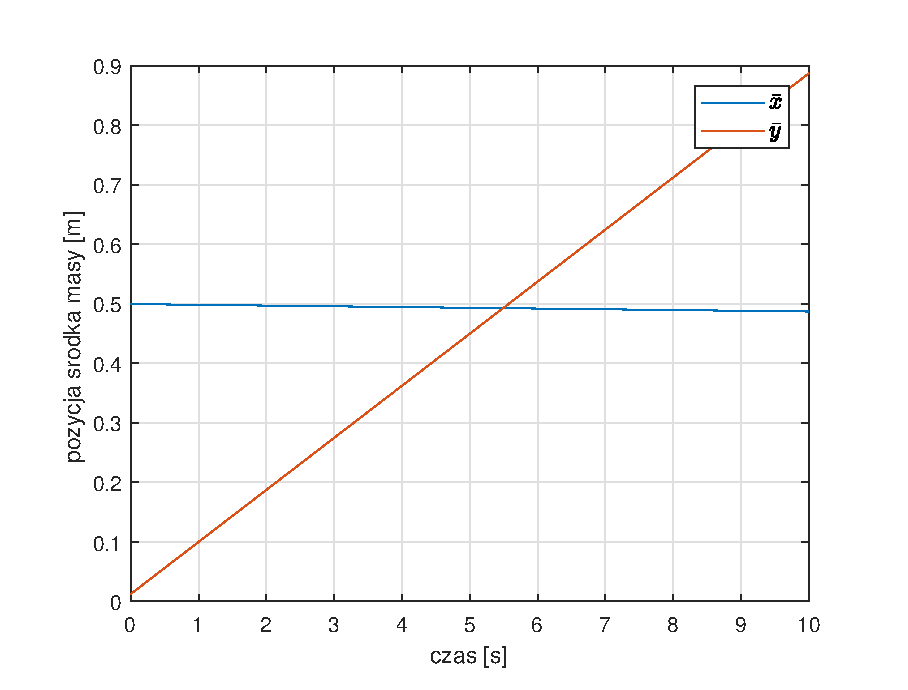
\includegraphics[width=.99\linewidth]{pics/FF1BaryXBAR}
\end{minipage}%
\begin{minipage}{.5\textwidth}
 	\centering
    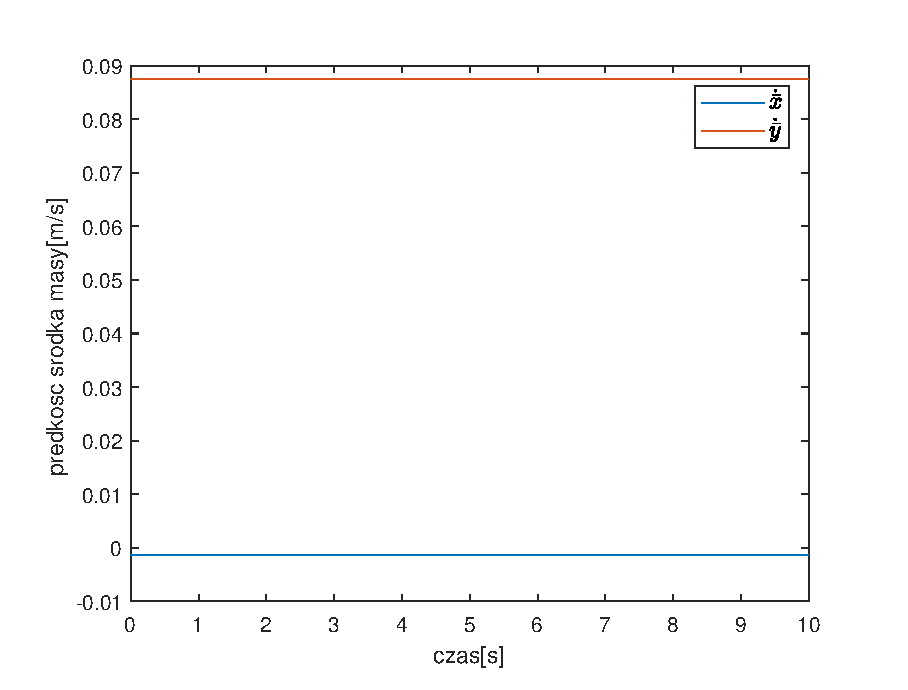
\includegraphics[width=.99\linewidth]{pics/FF1BaryXBARP}
\end{minipage}%
\caption{Przebiegi współrzędnych barycentrycznych $\bar{x}$ i $\bar{y}$ i ich prędkości}
\label{fig:FF1BaryXBAR}
\end{figure}

\end{document}
